\documentclass{article}

\usepackage{Sweave}
\begin{document}
\Sconcordance{concordance:analyzePower.tex:analyzePower.Rnw:%
1 2 1 1 0 7 1 1 14 5 0 1 2 1 3 5 0 1 2 1 3 5 0 1 2 3 1}


\title{Analyse der Akkulaufzeit}
\maketitle

\begin{figure}[H]
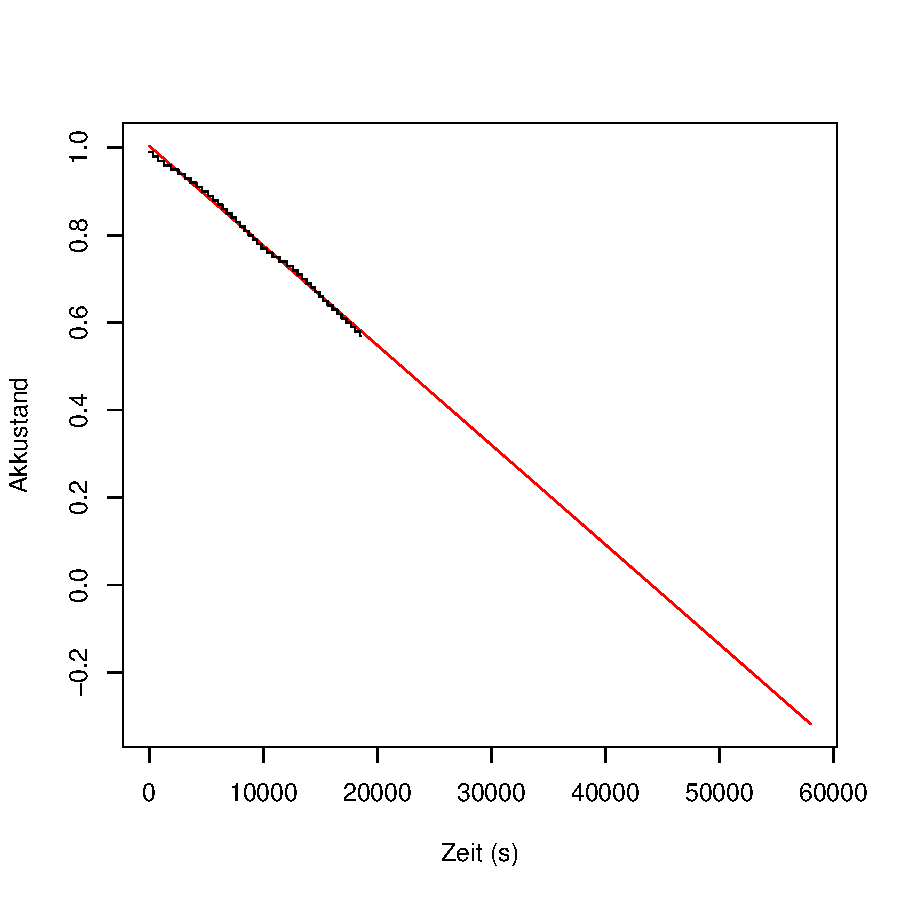
\includegraphics{analyzePower-001}
\caption{Beschleunigungsdaten, 1x pro Sekunde gespeichert}
\end{figure}


\begin{figure}[H]
\includegraphics{analyzePower-002}
\caption{Beschleunigungsdaten, 1x pro Minute gespeichert}
\end{figure}


\begin{figure}[H]
\includegraphics{analyzePower-003}
\caption{Gyro-Daten 1x pro Minute aufgezeichnet}
\end{figure}


\begin{figure}[H]
\includegraphics{analyzePower-004}
\caption{Beides 1x pro Sekunde gespeichert}
\end{figure}


\begin{figure}[H]
\includegraphics{analyzePower-005}
\caption{Beides 1x pro Minute gespeichert}
\end{figure}


\begin{figure}[H]
\includegraphics{analyzePower-006}
\caption{Noch mal zur Uebersicht}
\end{figure}

\end{document}
